\documentclass{beamer}
%\mode<presentation>
\usepackage[utf8]{inputenc}
\usepackage[magyar]{babel}
\usetheme{CambridgeUS}
\usecolortheme{dolphin}
\usepackage{amsmath,amssymb,amsfonts, bm}
\usepackage{mathpazo}
\usepackage{graphicx,tabularx,epsfig}
\usepackage[compatibility=false]{caption}
\usepackage{subcaption}
\usepackage{rotating}
\usepackage{mathtools}


\setbeamertemplate{background}{\tikz[overlay,remember picture]\node[opacity=0.07]at (current page.center){
\includegraphics[width=\paperwidth]{pic/bkg}};}
\usepackage{tikz}

\DeclareGraphicsExtensions{.pdf,.png,.jpg,.svg}


\setbeamertemplate{itemize items}[square]
\setbeamertemplate{enumerate items}[square]

\definecolor{Red}{RGB}{190,0,0}
\definecolor{Blue}{RGB}{0,0,190}
\setbeamertemplate{headline}{}



\title[Háromrészecske BE korrelációk vizsgálata]{ ÚNKP ÖSZTÖNDÍJASAINAK KONFERENCIÁJA \vspace{0.4cm}\\ Háromrészecske Bose-Einstein korrelációk vizsgálata}
\author[Bagoly Attila]{\Large{ Bagoly Attila}\\ \vspace{0.1cm}}
\date[2017. május 5.]{2017. május 5.}
\institute[ELTE TTK]{
\large{Témavezető: Csanád Máté}
}

\begin{document}

\begin{frame}
\vspace*{-20pt}
\begin{figure}

\includegraphics[scale=0.1]{pic/BNL2}
\hspace*{90pt}
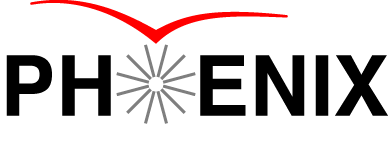
\includegraphics[scale=0.25]{pic/phenix}
\end{figure}
\vspace*{-30pt}
  \titlepage
\vspace*{-27pt}
\begin{figure}

\includegraphics[scale=0.05]{pic/ELTE}
\end{figure}

\end{frame}

\begin{frame}
\begin{itemize}
\frametitle{Áttekintés}
\setlength{\itemsep}{14pt}
\item Kutatás során nehézion ütközésekből származó adatok analízise történt
\item Gyorsító: Brookhaven nemzeti laboratorium relativisztikus nehézion ütköztetője (BNL RHIC)
\item Adatfelvétel: 2010, 200 GeV Au+Au ütközések
\item Mérés: PHENIX detektorrendszer
\item Adatmennyiség: 2.3 TB
\item Eredmények Quark Matter 2017 konferencián kerültek bemutatásra
\end{itemize}
\end{frame}

\section{HBT}
\begin{frame}
\frametitle{HBT effektus}
\begin{itemize}
\setlength{\itemsep}{8pt}
\item 1956. Robert Hanbury Brown és Richard Q. Twiss: A test of a new
type of stellar interferometer on Sirius
\item Két photomultiplier, különböző távolságok $\Rightarrow$ korreláció a két mért intenzitáseloszlásban
\item Korrelációs függvény a detektor távolság függvényében $\rightarrow$ Sirius átmérője
\end{itemize}
\begin{figure}
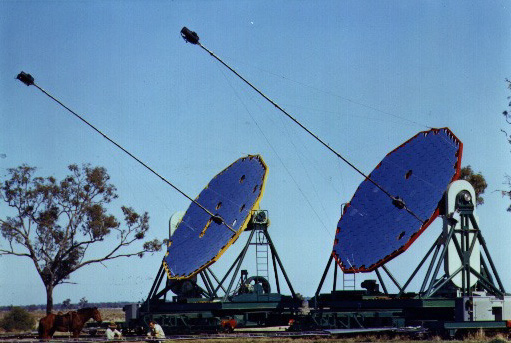
\includegraphics[scale=0.4]{pic/hbtdet.jpg}
\end{figure}
\end{frame}

\section{HBT effektus a részecskefizikában}
\begin{frame}
\frametitle{HBT effektus a részecskefizikában}
\begin{itemize}
\setlength{\itemsep}{14pt}
\item  1959. G. Goldhaber, S. Goldhaber, W.Y. Lee and A. Pais:
proton-antiproton ütközések 1.05 GeV/c energián:\vspace*{0.2cm}
\begin{itemize}
\setlength{\itemsep}{10pt}
\item vizsgálták $\rho^0\rightarrow \pi^+\pi^-$ bomlást
\item nem várt korreláció a $\pi^+$ és $\pi^+$, $\pi^-$ és $\pi^-$
\item 1960: oka pionok bozonok mint a fotonok
\end{itemize}
\item Később kiderült, hogy a korrelációk információt hordoznak a forrás geometriájáról
\item 200 GeV Au+Au ütközésekben a RHIC gyorsítóban kvark-gluon plazma keletkezik
\item Ennek az ``ősanyagnak'' a tulajdonságait vizsgáljuk a belőle kifagyott pionok közti korreláció mérésével
\end{itemize}
\end{frame}

\begin{frame}
\frametitle{Háromrészecske Bose-Einstein korrelációk }
\begin{itemize}
\setlength{\itemsep}{8pt}
\item Invariáns momentum eloszlás: $N_1(p_i), N_2(p_1,p_2),N_3(p_1, p_2, p_3)$
\item Korrelációs függvény definíciója:
\begin{equation*}
C_n(p_1,\dots,p_n)=\frac{N_n(p_1,\dots,p_n)}{N_1(p_1)\cdots N_1(p_n)}
\end{equation*}
 kaotikus emisszió esetén:
\begin{equation*}
N_n(p_1,\dots,p_n)=\int \prod_{i=1}^{n}\mathcal{S}(x_i,p_i)|\Psi_{n}(\{x_i\})|^2 d^4x_1\dots d^4x_n
\end{equation*}
\item $\mathcal{S}(x,p)$ forrásfüggvény (általában Gaussian eloszlás - Levy általánosabb)
\end{itemize}
\end{frame}

\begin{frame}
\frametitle{Core-Halo modell}
\begin{itemize}
\setlength{\itemsep}{8pt}
\item nem minden részecske származik a QGP kifagyásból
\item már kifagyott részecskék bomlásából is származnak beütések
\item Mindkét rész hozzájárul a forrásfüggvényhez:
\begin{equation*}
\mathcal{S}=\mathcal{S}_{\rm core}+\mathcal{S}_{\rm halo}
\end{equation*}
\item Részecskeszám eloszlás:
\begin{equation*}
N_n(p_1,\dots,p_n) = N_n^{c}(p_1,\dots,p_n)+N_n^{h}(p_1,\dots,p_n)
\end{equation*}
\item Két részecske korreláció:
\begin{equation*}
C_2(k_1, k_2) =  1+\lambda_2|\mathcal{S}(q)|^2
\end{equation*}
ahol
\begin{equation*}
\sqrt{\lambda_2} =  f_C \equiv \frac{N^c}{N^c+N^h} 
\end{equation*}
\end{itemize}
\end{frame}

\begin{frame}
\frametitle{Koherencia}
\begin{itemize}
\setlength{\itemsep}{8pt}
\item Ha a mag részeben koherens módon kelt részecskéket:
\begin{equation*}
\mathcal{S}_{\rm core}=\mathcal{S}_{\rm core}^{\rm pc}+\mathcal{S}_{\rm core}^{i}
\end{equation*}
ahol pc a koherens részre, i az inkoherens részre utal
\item Részecskeszám eloszlás:
\begin{equation*}
N_n^{c}(p_1,\dots,p_n) = N_n^{c,{\rm pc}}(p_1,\dots,p_n)+N_n^{c, {\rm i}}(p_1,\dots,p_n)
\end{equation*}
\item Két részecske korreláció: $C_2(k_1, k_2) =  1+\lambda_2|\mathcal{S}(q)|^2$, de $\lambda_2 \neq f_C^2$
\item Koherensen keltett pionok aránya:
\begin{equation*}
p_C \equiv \frac{N_{\rm coherent}}{N^{\rm coherent}+N^{\rm incoherent}} \rightarrow \lambda_2(f_C, p_C)
\end{equation*}
\end{itemize}

\end{frame}

\section{Motiváció}
\begin{frame}
\frametitle{Háromrészecske HBT analízis mögötti motiváció}
\begin{itemize}
\setlength{\itemsep}{10pt}
\item Emlékeztető: $C_2(k) = 1 + \lambda_2 |\mathcal{S}(q)|^2$
\item Kétrészecske korreláció erőssége: $\lambda_2 \equiv C_2(q=0)-1$
\item Hasonlóan háromrészecske korrelációs erősség: $\lambda_3 \equiv C_3(0)-1$
\item Core-Halo: \vspace*{-15pt}
	\begin{align*}
		\lambda_2=f_C^2,\;\;\;\;\lambda_3 = 2f_C^3+3f_C^2 \\ 
		\kappa_3=\big(\lambda_3-3\lambda_2\big)/\big(2\sqrt{\lambda_2^3}\big)=1
	\end{align*}
\item Parciális koherencia ($p_C$ koherensen keltett pionok aránya): 
	\begin{gather*}
		\lambda_2=f_C^2\big[(1-p_C)^2+2p_C(1-p_C)\big]\\
		\lambda_3=2f_C^3\big[(1-p_C)^3+3p_C(1-p_C)^2\big]+3f_C^2\big[(1-p_C)^2+2p_C(1-p_C)\big]\nonumber\\
		\kappa_3 = \kappa_3(p_C)
	\end{gather*}
\item A $\lambda_2$, $\lambda_3$ konzisztens analíziséből vizsgálhatjuk az eltéréseket a Core-Halo modelltől
\end{itemize}
\end{frame}


\begin{frame}
\frametitle{Korrelációs függvény}
\begin{itemize}
\setlength{\itemsep}{10pt}
\item $C_3(p_1,p_2,p_3)$ (9D) 

\item különböző $p_T=|p_{T1}+p_{T2}+p_{T3}|/3$ binekben mérjük a $C_3(k_{12}, k_{23}, k_{13})$ (6D) függvényt, ahol $k_{ij}=p_i-p_j$ 
\item side-out-longitudinal felbontást használunk:
\begin{itemize}
\setlength{\itemsep}{4pt}
\item long irány: nyalábirány
\item out irány: átlagos transzverz irány 
\item side: merőleges előző kettőre
\end{itemize}
\item Koordináta rendszer: háromrészecske LCMS (longitudinális együttmozgó rendszer): Lorentz boost long irányba
\item A $\bm{k_{ij}^{\mathrm{LCMS}}}$ helyett a korrelációs függvényt változói:
\begin{equation*}
k_{ij}=|\bm{k_{ij}^{\mathrm{LCMS3}}}|\;\;\;\;\;\;\;\;\;\;\;\;\;(3D)
\end{equation*}
\item Ok: nincs elég statisztika
\end{itemize}
\end{frame}


%\begin{frame}
%\frametitle{Mérés részletei}
%\begin{itemize}
%\setlength{\itemsep}{14pt}
%\item BNL RHIC, PHENIX kísérlet, 200GeV Au+Au ütközések
%\item Esemény-keverő módszer a korrelációk mérésére: momentum különbség eloszlás azonos eseményből, háttér ugyanez csak különböző eseményekből 
%\item MinBias: nincs centralitás szűrés
%\end{itemize}
%\begin{figure}
%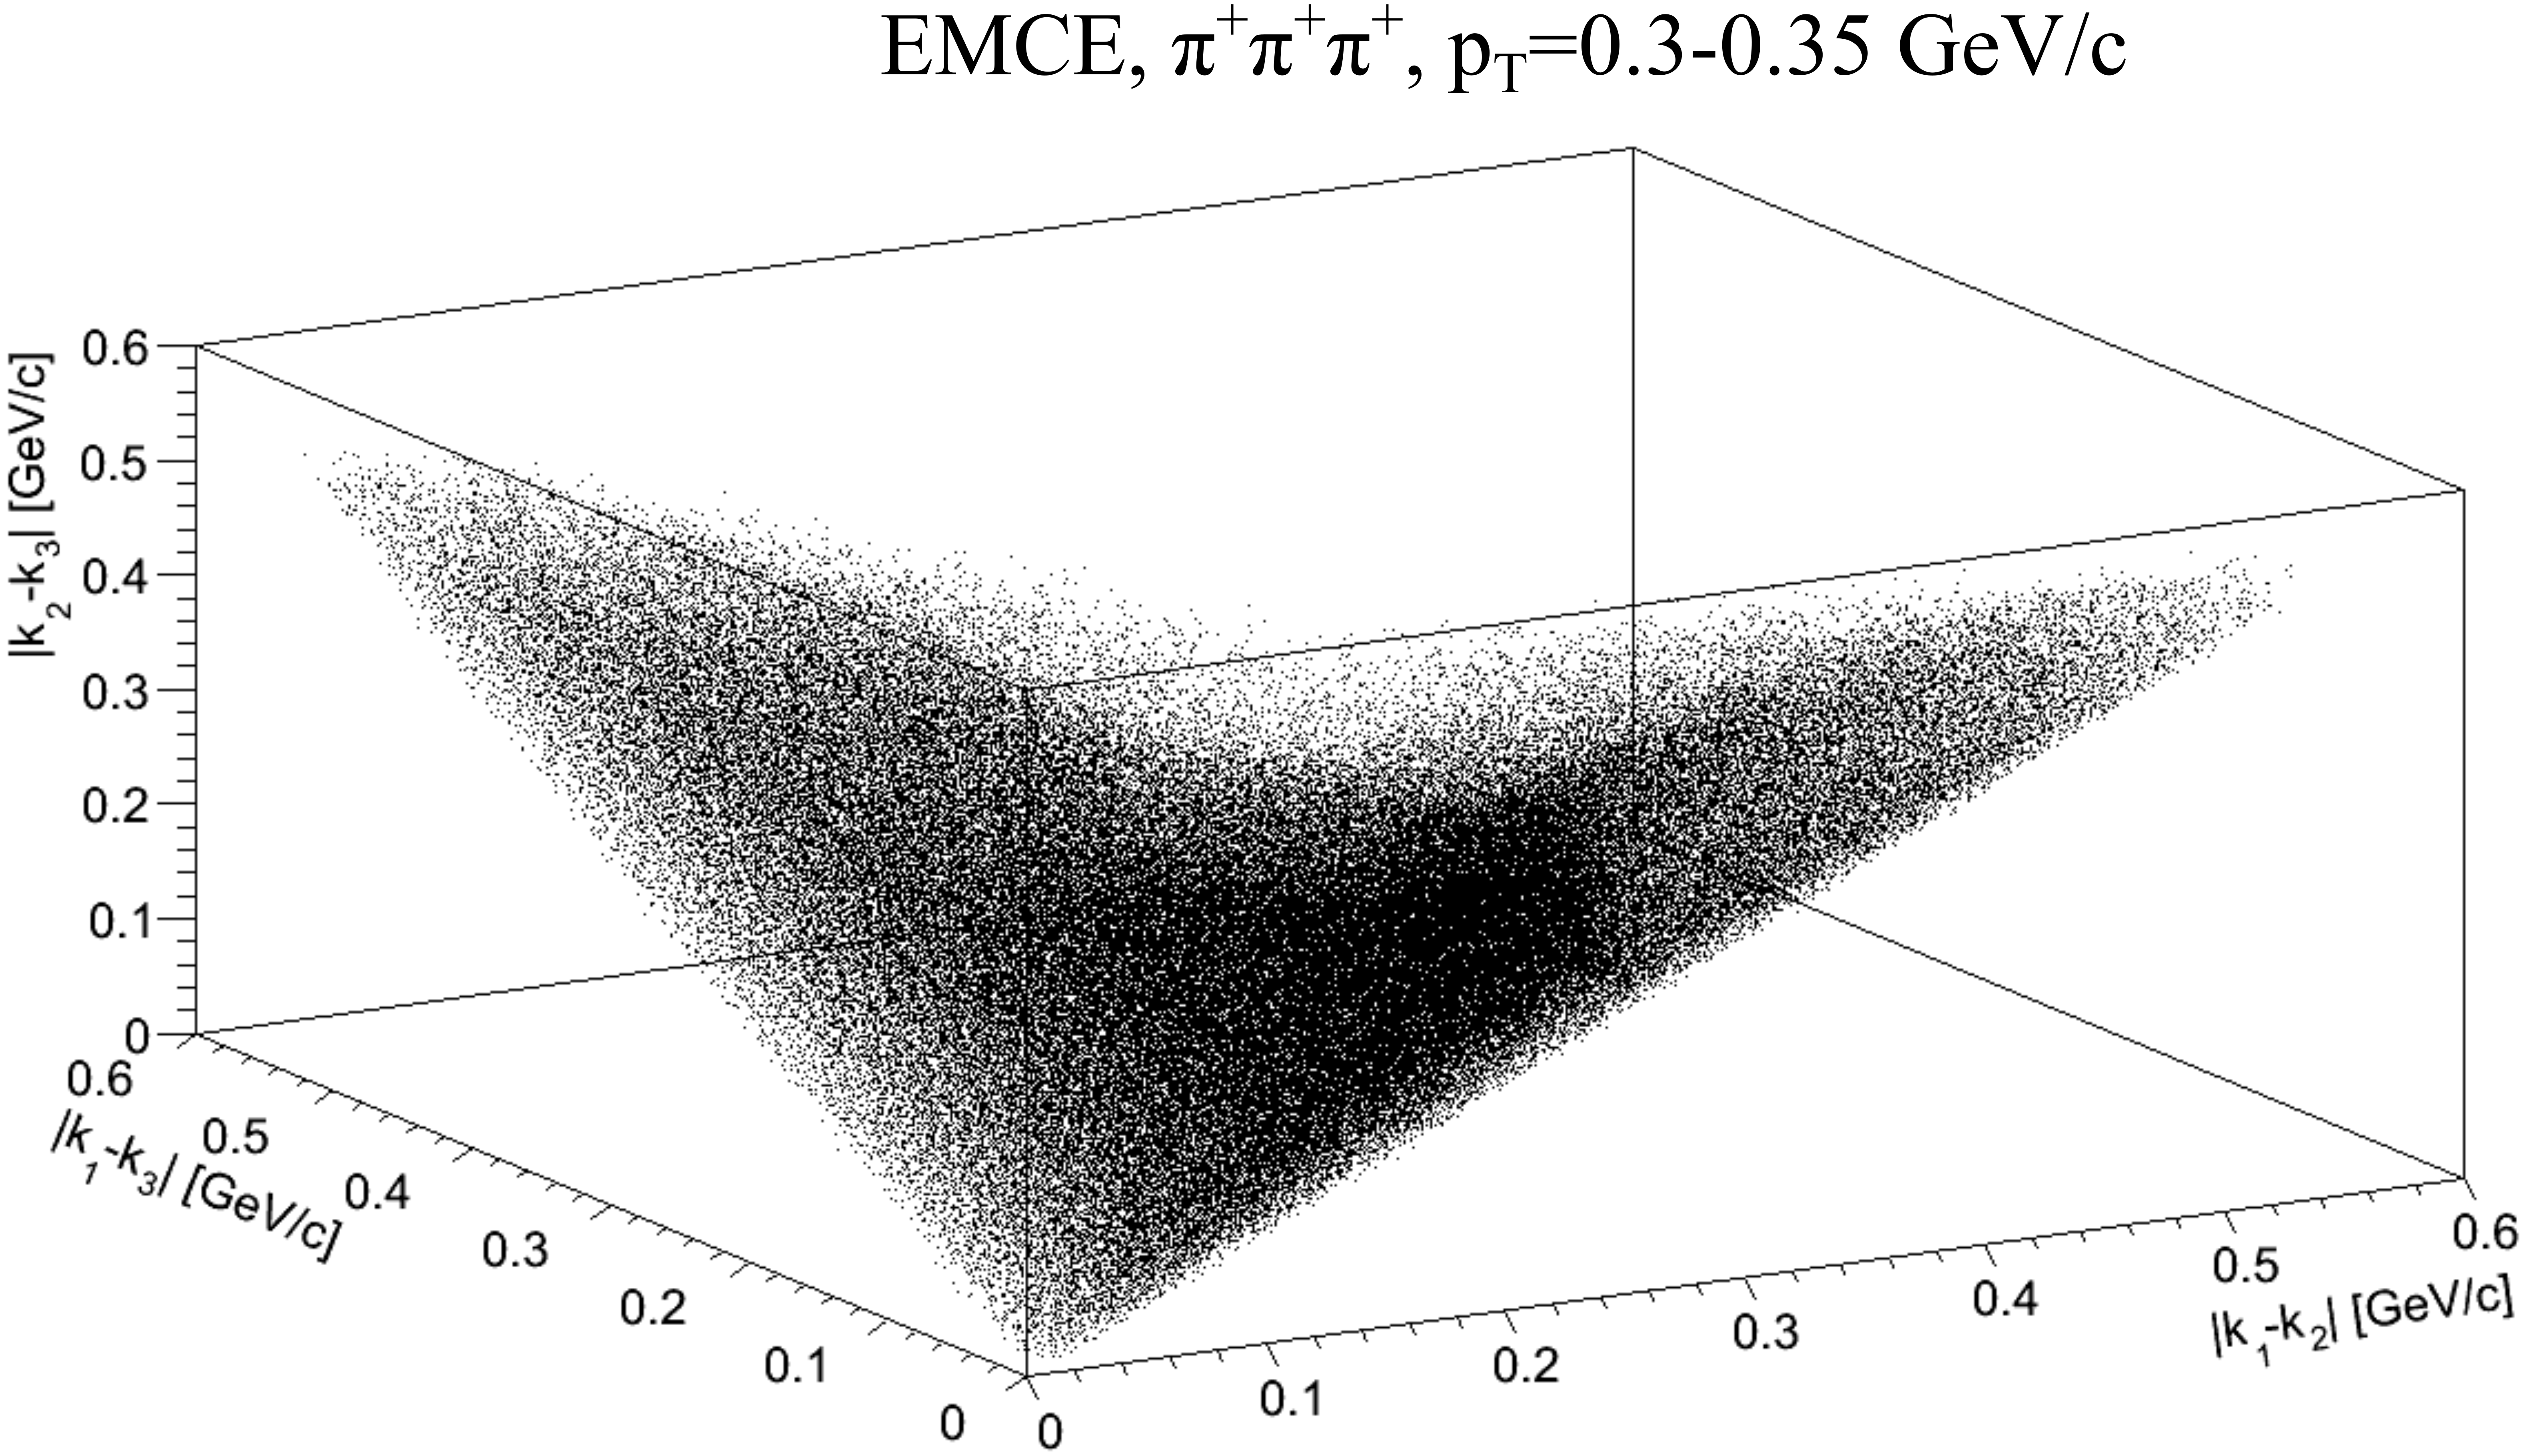
\includegraphics[scale=0.05]{pic/C1}
%\end{figure}
%\end{frame}



\section{Model}
\begin{frame}
\frametitle{Coulomb kölcsönhatás nélküli modell}
\begin{itemize}
\setlength{\itemsep}{12pt}
\item Feltevés a forrásra: Levy-eloszlás
\begin{equation*}
\mathcal{L}(\alpha,R,r)=(2\pi)^{-3} \int d^3q e^{iqr} e^{-\frac{1}{2}|qR|^{\alpha}}
\end{equation*}
\item $C_3$ közelíthető a következőképpen ($\mathcal{L}_3=2f_C^3$):
\begin{align*}
C_3^{(0)}(k_{12}, k_{13}, k_{23}) = 1+ \ell_3e^{-0.5(|2k_{12}R_C|^\alpha+|2k_{13}R_C|^\alpha+|2k_{23}R_C|^\alpha)}\nonumber\\
+\ell_2\bigg(e^{|2k_{12}R_C|^\alpha}+e^{|2k_{13}R_C|^\alpha}+e^{|2k_{23}R_C|^\alpha}\bigg)
\end{align*}
\item Háttér: $N(1+\epsilon k_{12})(1+\epsilon k_{13})(1+\epsilon k_{23})$
\item Illesztési paraméterek: $\ell_3$, $\ell_2$,  $R_C$, $\alpha$, $N$, $\epsilon$
\item Keressük: $\lambda_3 \equiv  C_3(k_{12}=k_{13}=k_{23}=0)-1=\ell_3+3\ell_2$
\end{itemize}
\end{frame}

\begin{frame}
\frametitle{Coulomb korrekció}
\begin{itemize}
\setlength{\itemsep}{12pt}
\item Korrigált modell:
\begin{equation*}
C_3(k_{12}, k_{13}, k_{23}) = C_3^{(0)}(k_{12}, k_{13}, k_{23})\cdot K_3(k_{12}, k_{13}, k_{23})
\end{equation*}
\item ''Generalized Riverside'' közelítő módszer a Coulomb korrekció becslésére:
\begin{equation*}
K_3(k_{12}, k_{13}, k_{23}) \approx K_1(k_{12})K_1(k_{13})K_1(k_{23})
\end{equation*}
\end{itemize}
\vspace*{-20pt}
\begin{figure}
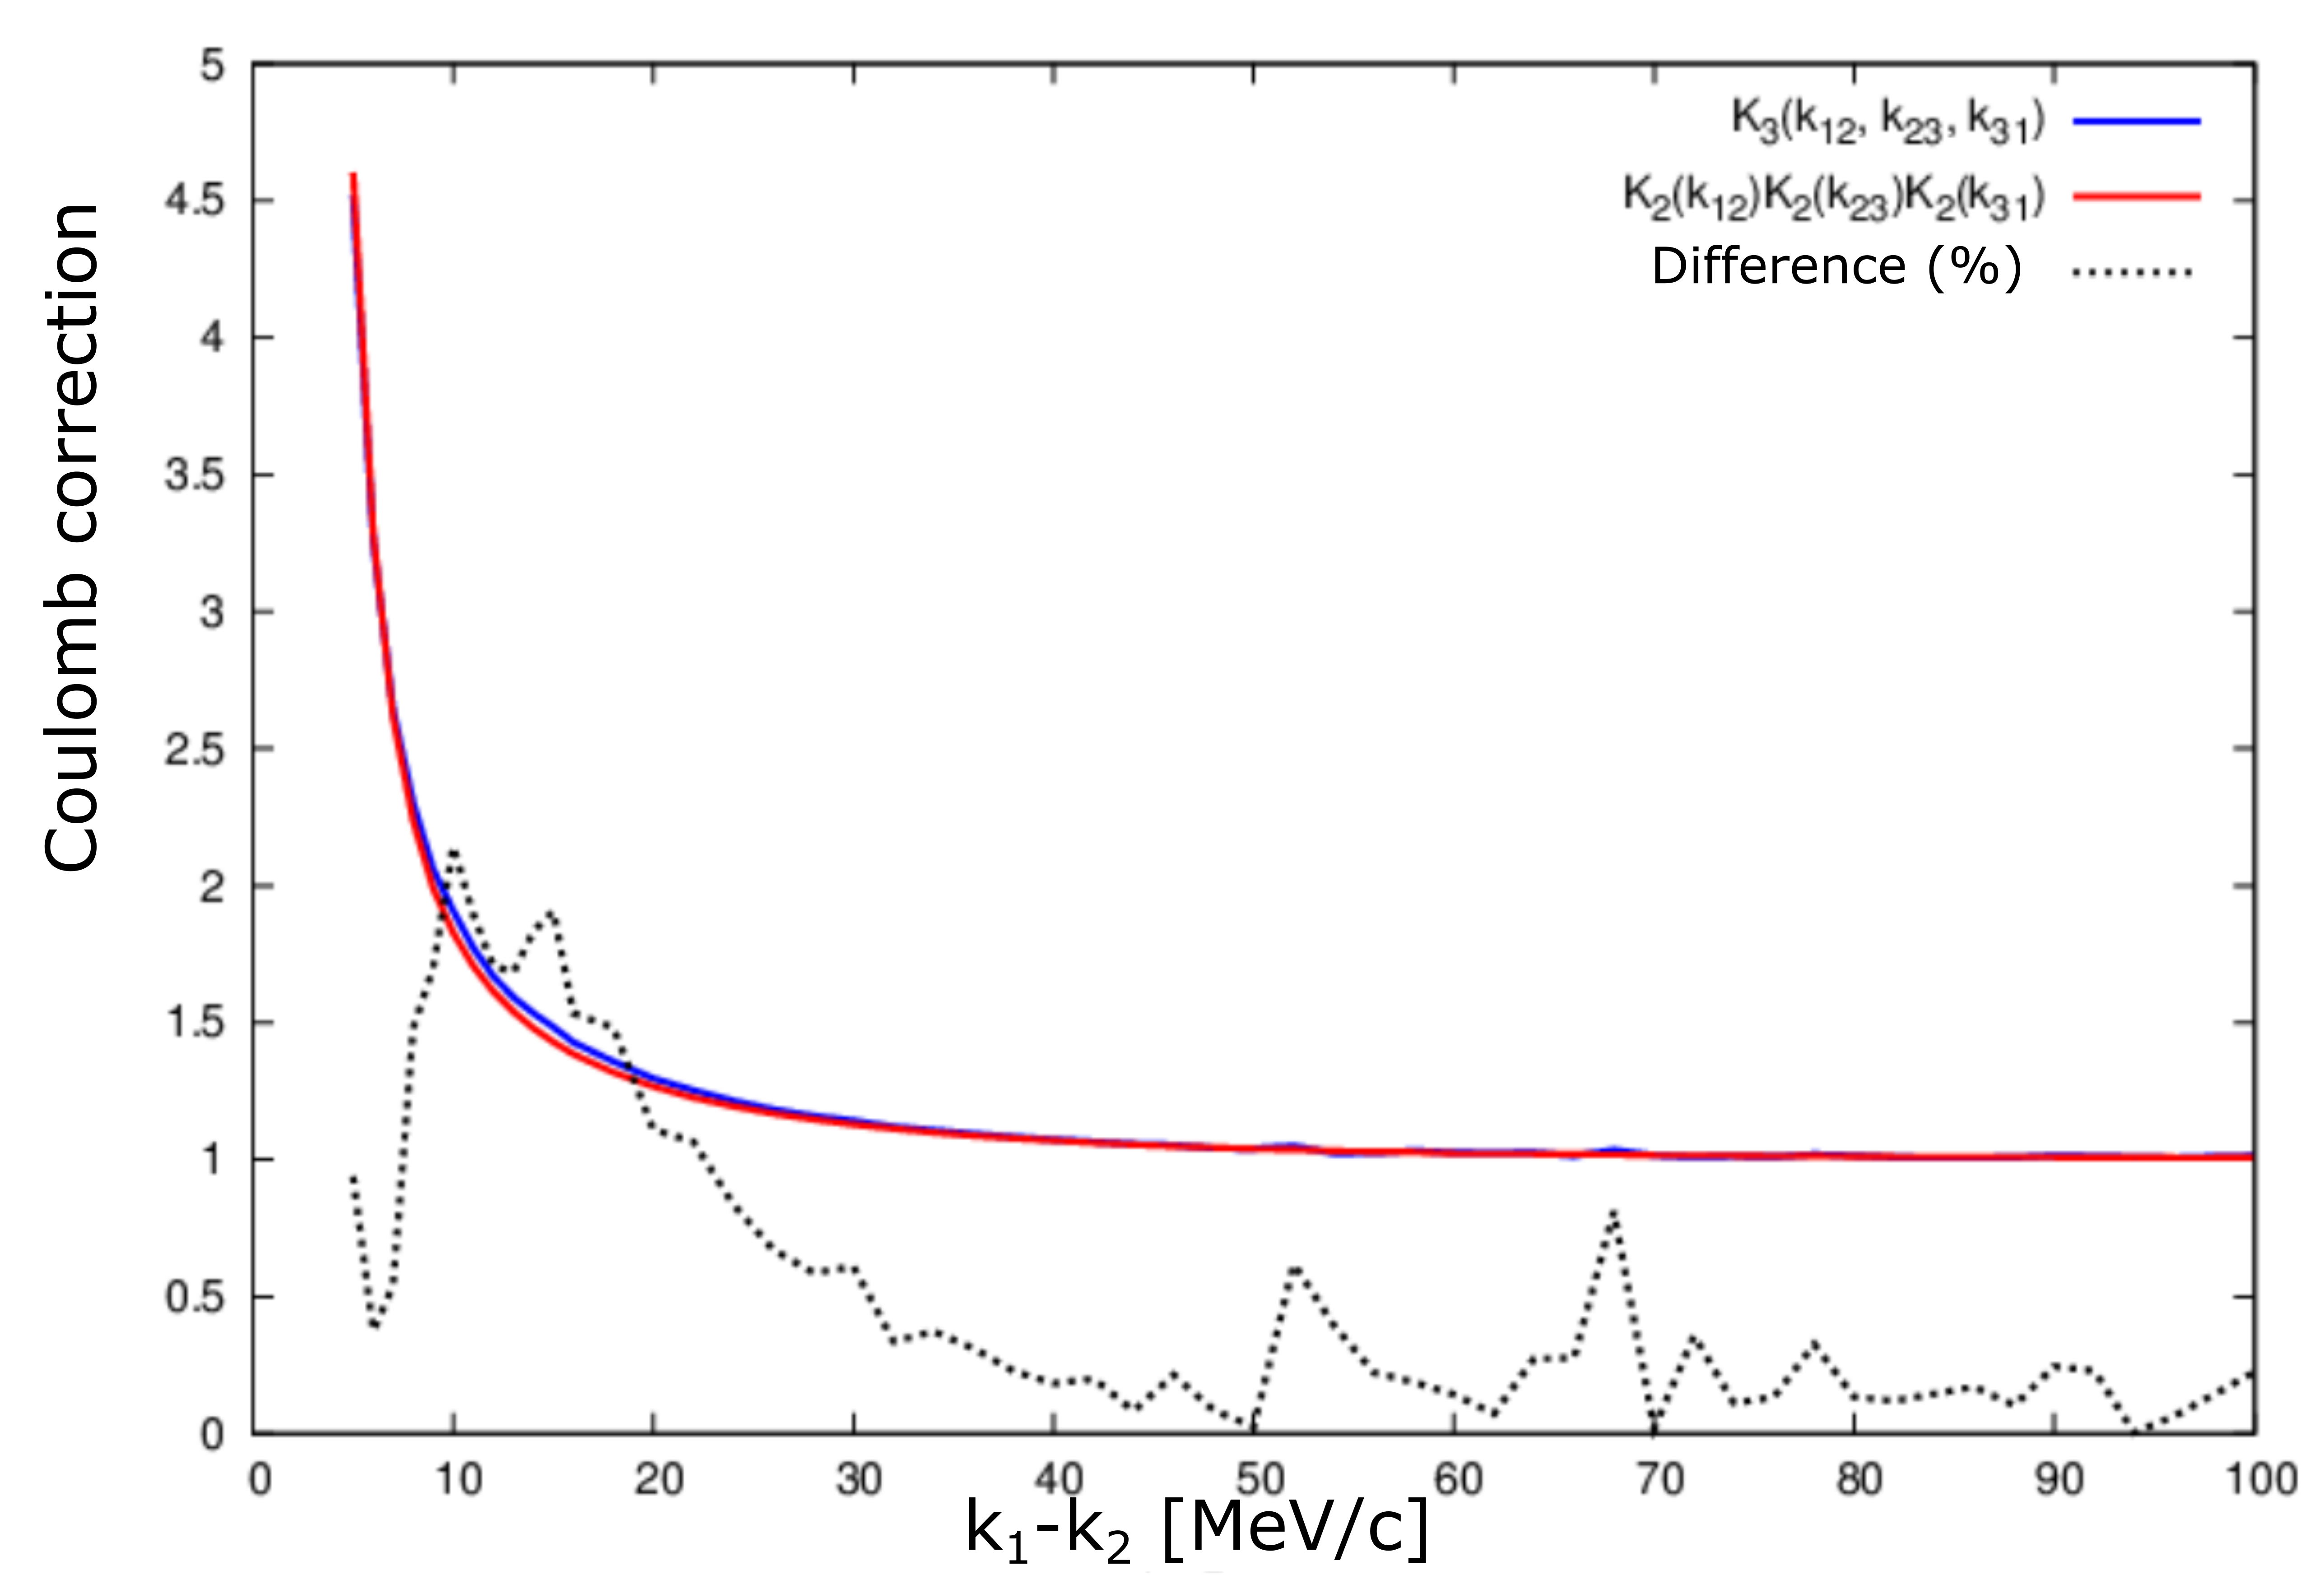
\includegraphics[scale=0.25]{pic/coulomb1}
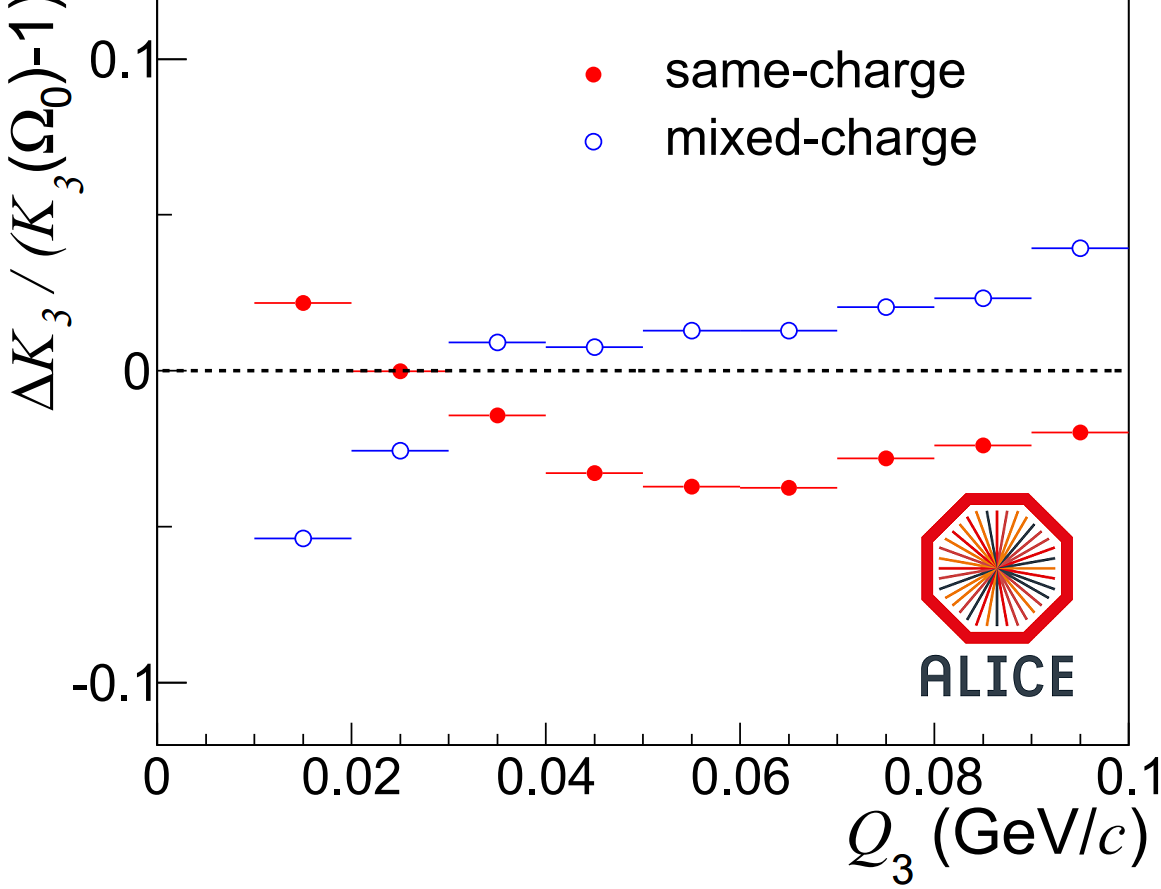
\includegraphics[scale=0.235]{pic/coulomb2}
\end{figure}
\end{frame}

\begin{frame}
\frametitle{Illesztés szemléltetése}
\begin{itemize}
\setlength{\itemsep}{16pt}
\item Diagonális korrelációs függvény
\end{itemize}
\begin{figure}
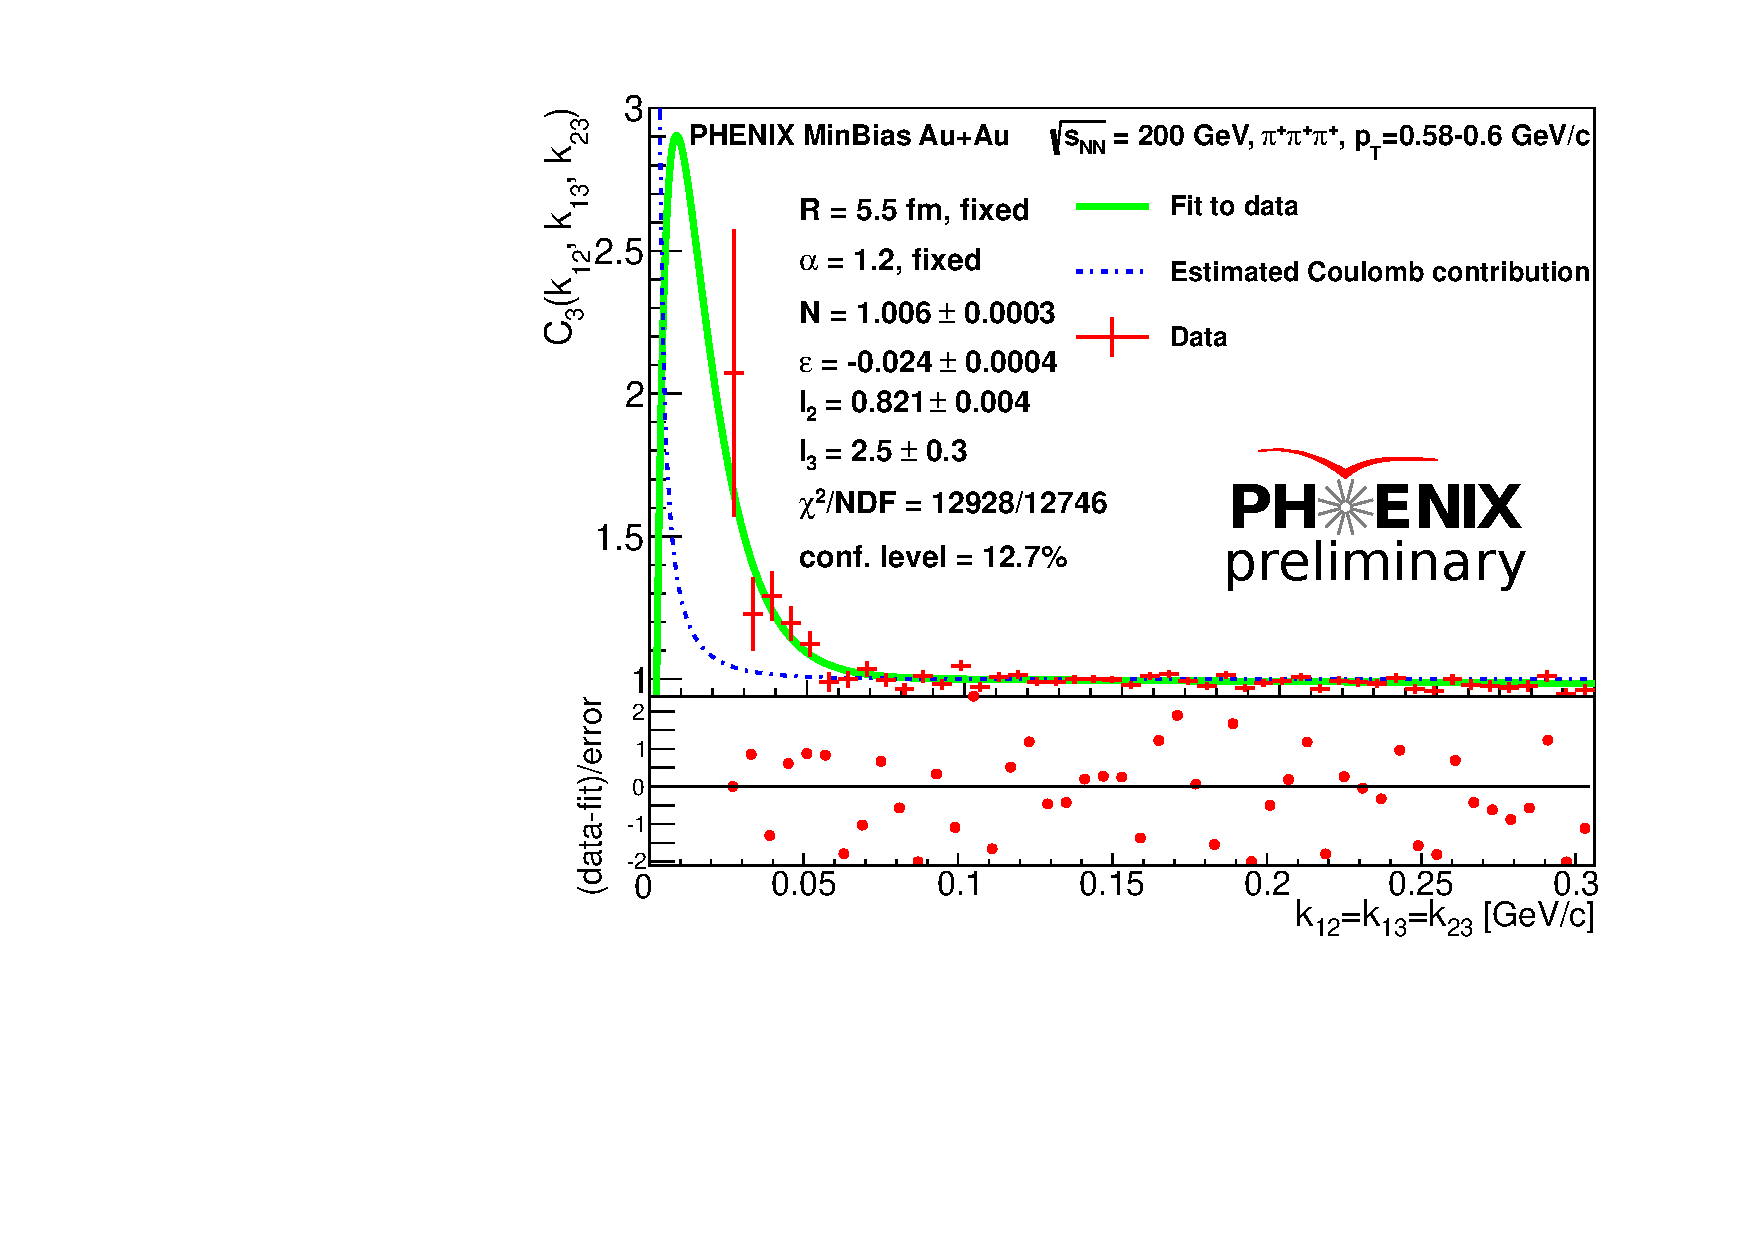
\includegraphics[scale=0.45]{pic/diag_highpt.pdf}
\end{figure}
\end{frame}

\begin{frame}
\frametitle{Háromrészecske korrelációs erősség: $\lambda_3$}
\begin{itemize}
\setlength{\itemsep}{10pt}
\item $\lambda_3$ Core-Halo  + kaotikus forrás által adott tartományban minden $m_T$
\end{itemize}
\begin{figure}
\colorbox{white}{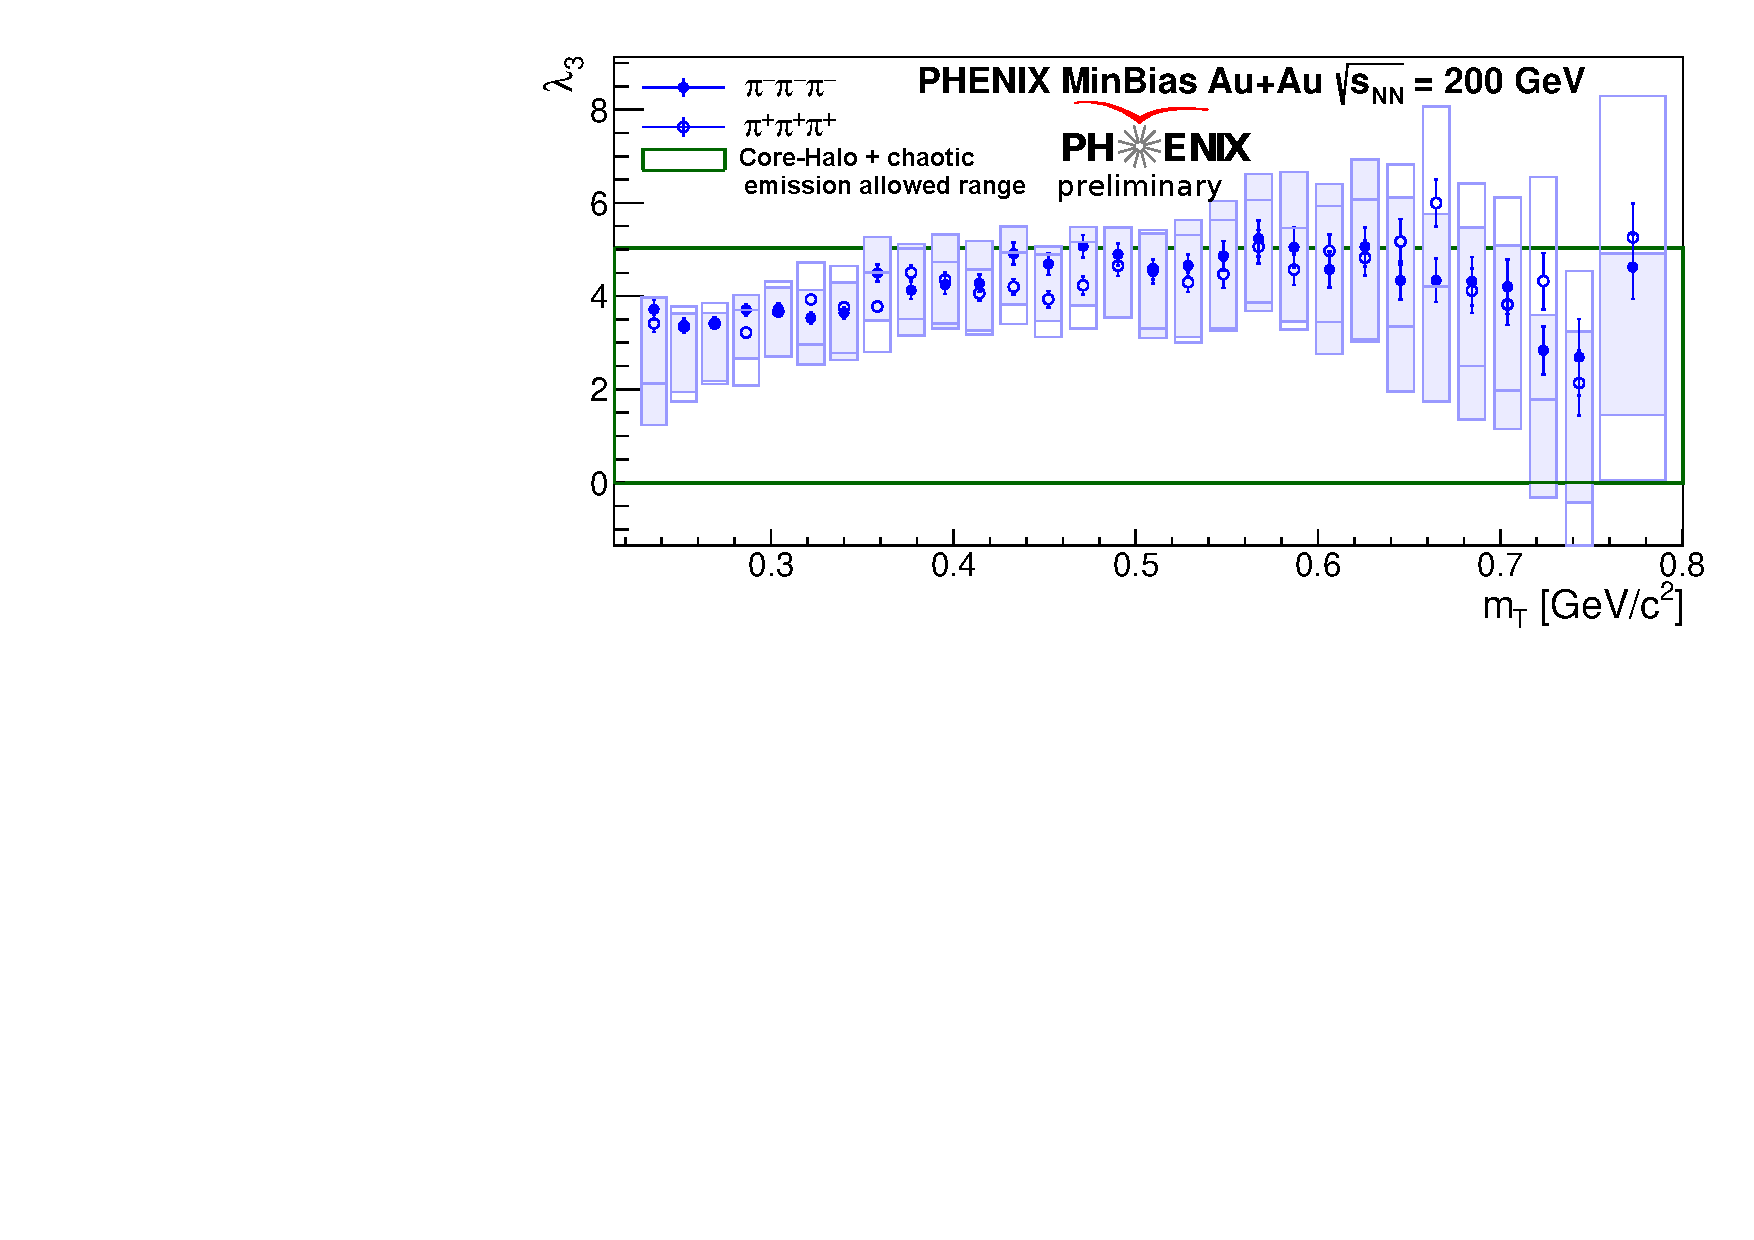
\includegraphics[scale=0.6]{pic/lambda3}}
\end{figure}
\end{frame}



\begin{frame}
\frametitle{Core-Halo független paraméter}
\begin{itemize}
\item $\kappa_3\equiv\frac{\lambda_3-3\lambda_2}{2\sqrt{\lambda_2^3}}$ nem függ $f_C$-től ($f_C=\mathrm{core}/(\mathrm{core}+\mathrm{halo})$)
\item Core-Halo + kaotikus mag: $\kappa_3=1$
\item új effektusok (pl. nem teljesen kaotikus forrás): $\kappa_3\neq 1$
\item Statisztikailag szignifikáns eltérés a $\kappa_3=1$
\end{itemize}
\begin{figure}
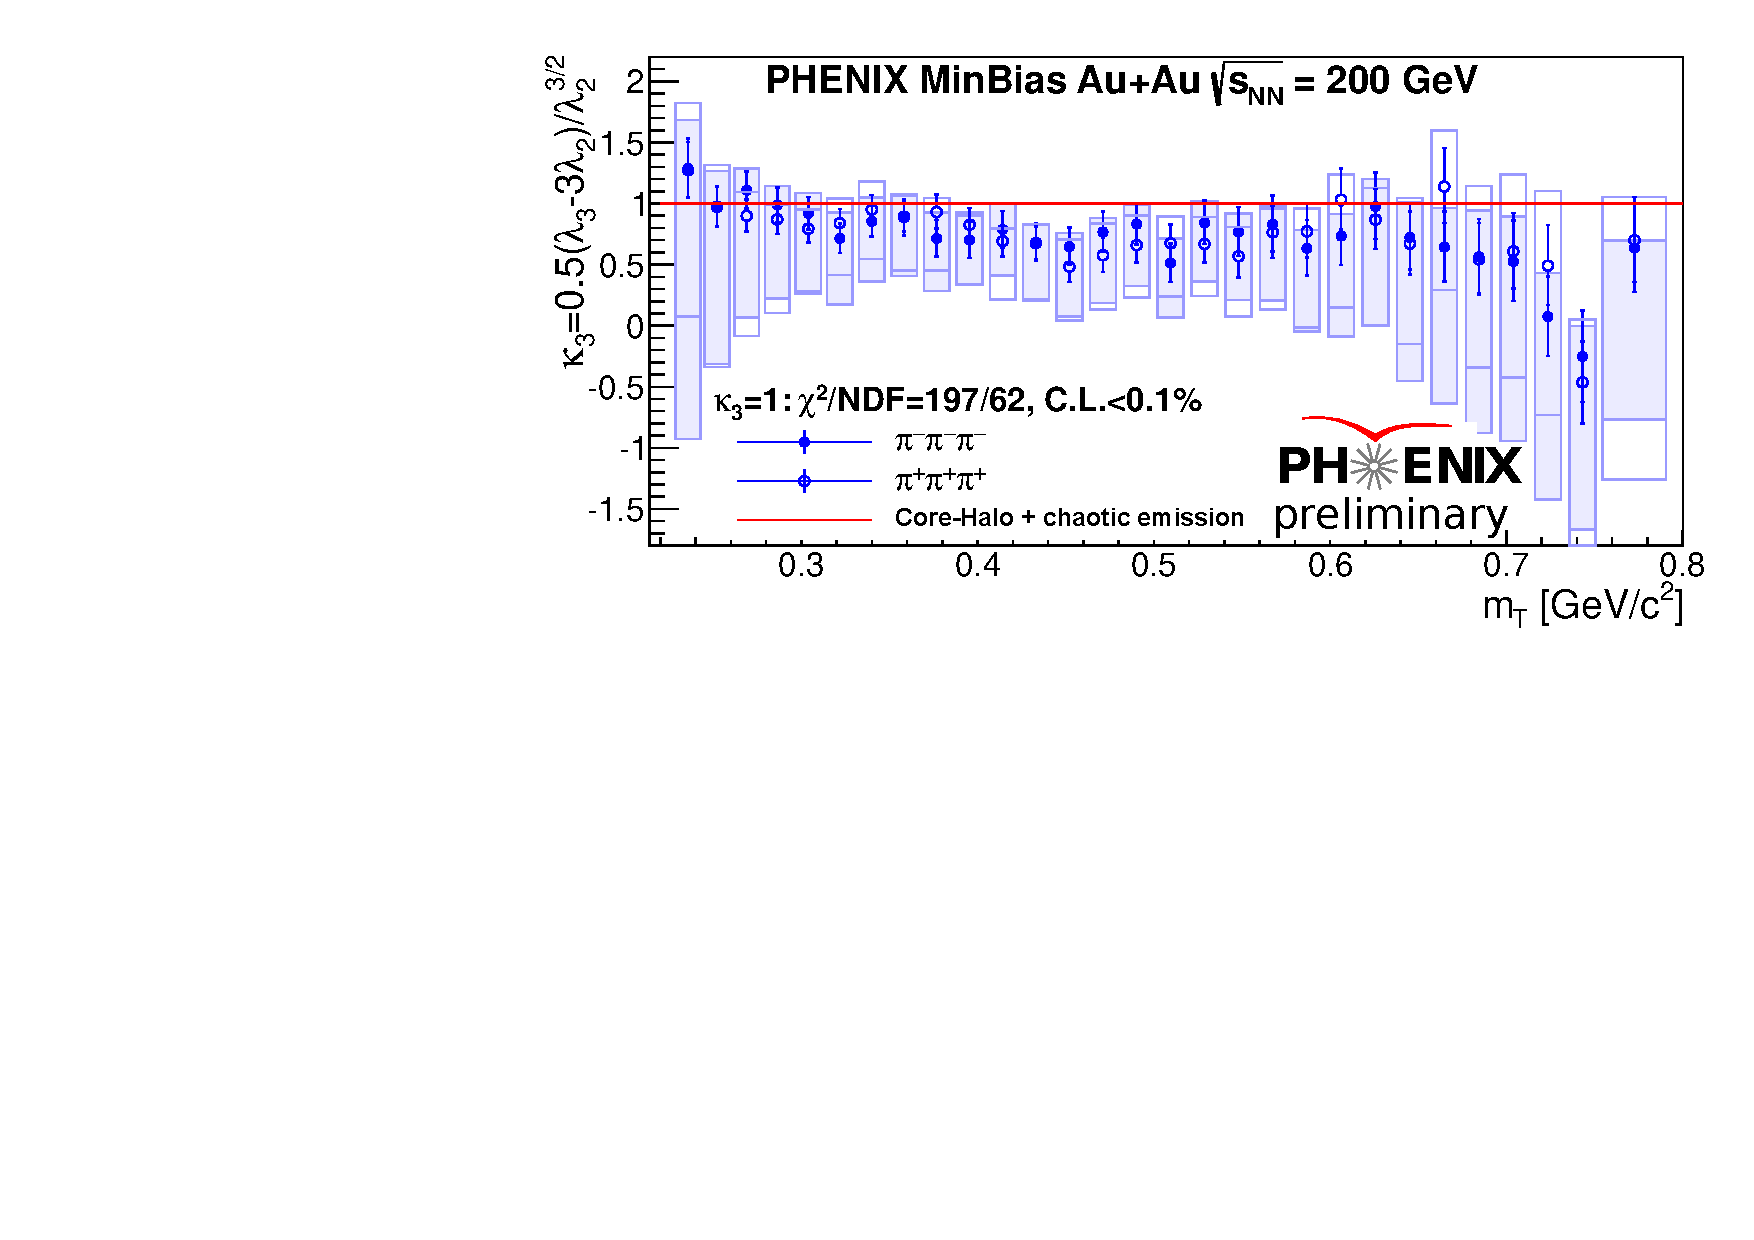
\includegraphics[scale=0.5]{pic/kappa3}
\end{figure}
\end{frame}


\begin{frame}
\frametitle{Mag aránya ($f_c$) a parciális koherencia ($p_c$) függvényében}
\begin{itemize}
\vspace{-0.004\textheight}
\item Egyszerű elméleti modell: $\lambda_2(f_c, p_c)$, $\lambda_3(f_c, p_c)$ 
\item Mért $\lambda_2^{\rm meas.} \rightarrow \lambda_2^{\rm meas.}=\lambda_2(f_c,p_c) \Longrightarrow f_c(p_c)$ (zöld vonalak)
\item Mért $\lambda_3^{\rm meas.} \rightarrow \lambda_3^{\rm meas.}=\lambda_3(f_c,p_c) \Longrightarrow f_c(p_c)$ (kék vonalak)
\item $f_c<0.82$ és $p_c>0.5$ kizárható, $p_C<0.5$ nem zárható ki
\end{itemize}

\begin{figure}
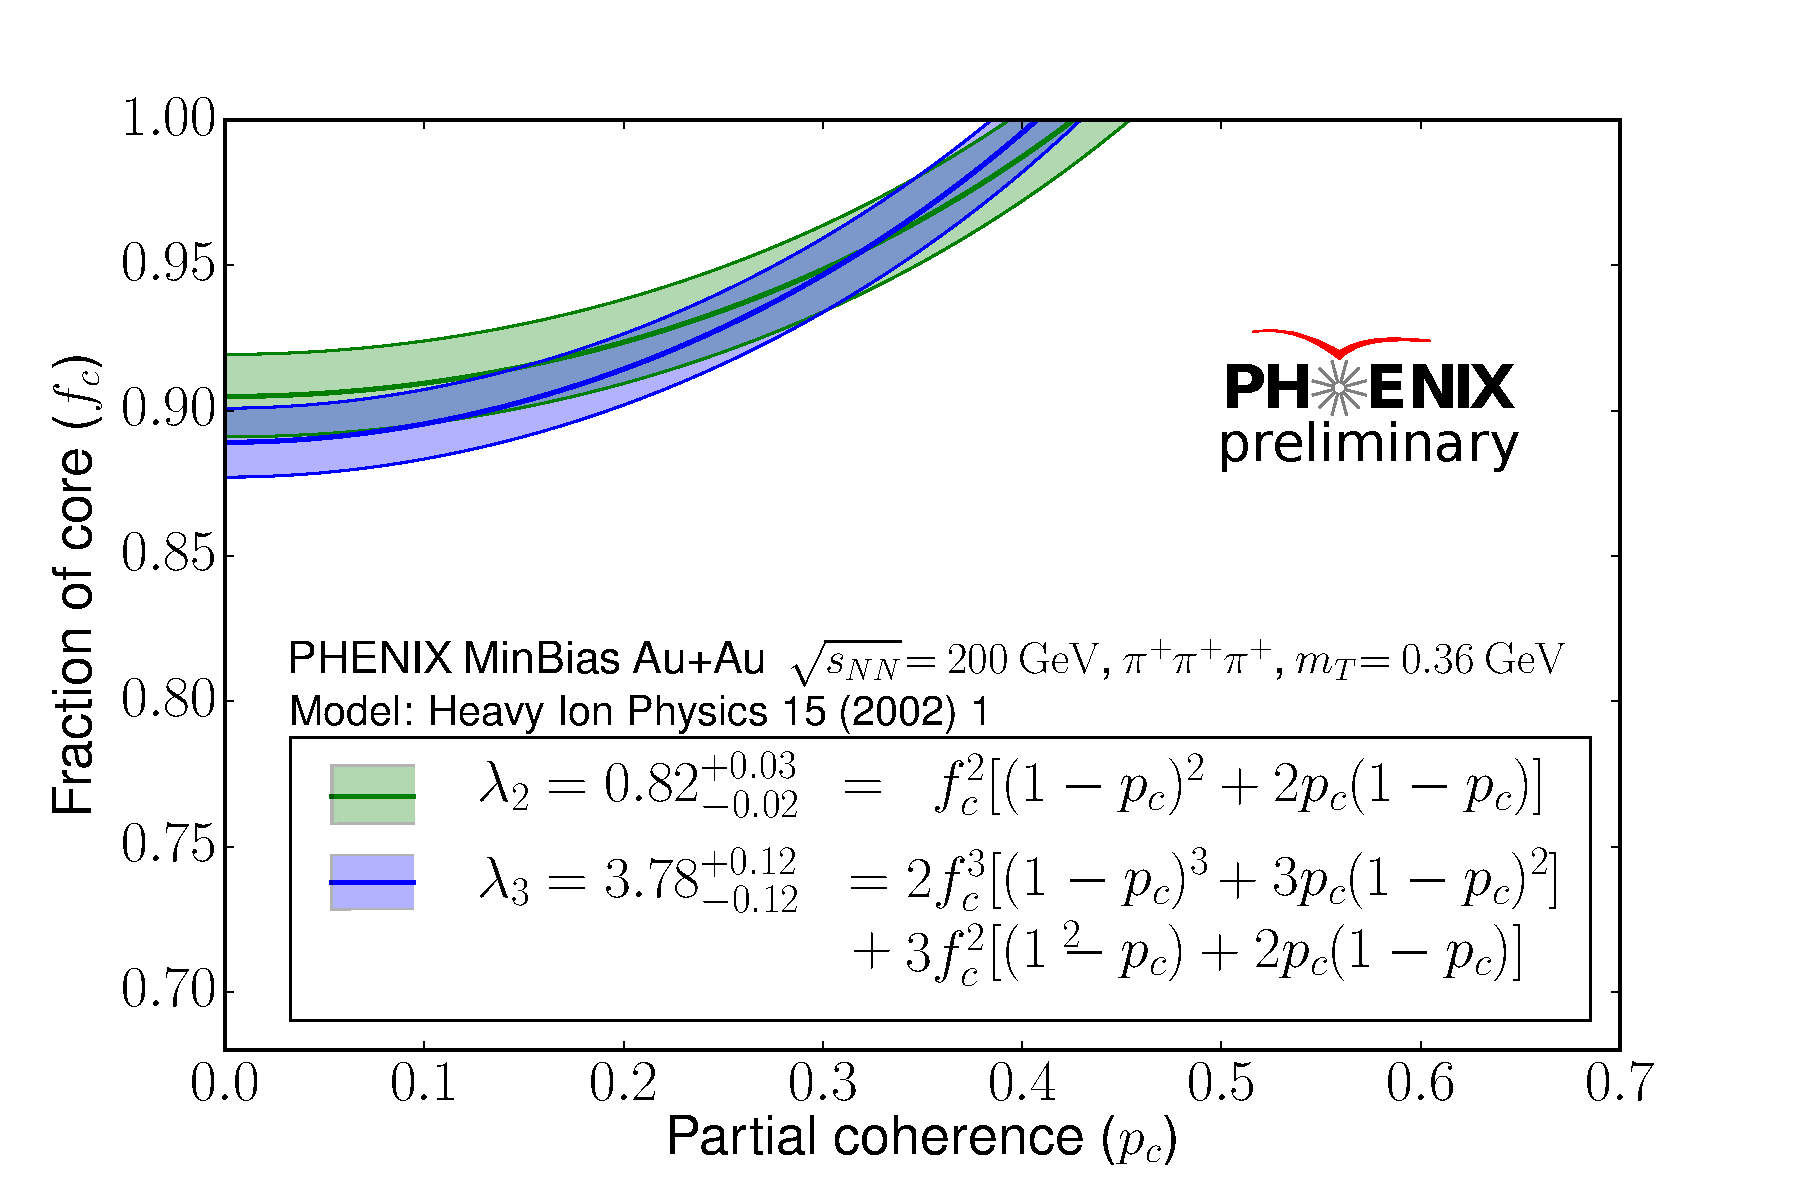
\includegraphics[width=0.7\textwidth]{pic/cropped_fcpc2}
\end{figure}
\end{frame}

\begin{frame}
\frametitle{Összefoglaló}
\begin{itemize}
\setlength{\itemsep}{10pt}
\item RHIC gyorsító 200GeV Au+Au ütközések során a PHENIX detektorrendszerrel mért adatok analízisét végeztem
\item Háromrészecske korrelációs függvényeket mértem
\item Korrelációs függvény modelljében forrás leírására: Lévy eloszlás
\item A cél a háromrészecske korreláció erősségének meghatározása volt
\item Kétrészecske és háromrészecske korrelációs erősségek analíziséből kiderült:
\begin{itemize}
	\item statisztikailag szignifikáns eltérés az egyszerű Core-Halo + kaotikus mag modelltől
	\item $82\%$-nál kisebb magarány és $50\%$-nál nagyobb koherencia kizárható a vizsgált $p_T$-n
	\item $50\%$-nál kisebb koherencia nem zárható ki az analízis alapján
\end{itemize}
\end{itemize}
\end{frame}

\end{document}

